
\chapter{\textbf{Metodologia}}\label{cap:metodologia}
    \section{Coleta e Seleção de Dados}\label{sec:coleta}
        Esse estudo adota uma abordagem descritiva de pesquisa para examinar e interpretar certos métodos de cálculo de massa estelar quantitativamente, fazendo o uso de ferramentas estatísticas para aferir a qualidade das determinações e estimativas realizadas. A seleção da amostra é não probabilística, caracterizada pela escolha deliberada dos elementos a serem incluídos, dado o foco maior para estrelas jovens de baixa massa. 
            
        Para estudar os aglomerados estelares, foram utilizados os catálogos presentes em \citeonline{hillenbrand1997stellar}, \citeonline{cieza2007testing}, \citeonline{davies2014accretion}, \citeonline{kounkel2022untangling} para a ONC, \citeonline{lodieu2019fiveD} para as Plêiades, \citeonline{rebull2018rotation} e \citeonline{stauffer2019rotational} para o USco, \citeonline{moraux2013monitor} para a NGC 869 e \citeonline{jackson2012why} para a NGC 2516.
        
		Alguns parâmetros complementares necessários para esse estudo foram obtidos a partir dos catálogos do GAIA \cite{gaia2022, gaia2022b} e TESS \cite{paegert2021tessinputcatalogversions}. O GAIA é uma missão espacial da Agência Espacial Europeia (ESA) dedicada a mapear com alta precisão a paralaxe, o movimento próprio as e características fotométricas de mais de um bilhão de estrelas na Via Láctea. Seus dados são essenciais para a estimativa de distâncias e para o estudo da estrutura e evolução galáctica. Já o TESS (Transiting Exoplanet Survey Satellite) é uma missão da NASA que tem como principal objetivo detectar exoplanetas por meio do método de trânsito, mas também fornece dados fotométricos de alta qualidade para milhões de estrelas. Os dados do TESS são especialmente úteis para estudar variações de brilho, permitindo análises detalhadas de variabilidade estelar e a identificação de objetos de interesse astrofísico. Esses dois catálogos, portanto, são fundamentais para enriquecer a análise dos parâmetros estelares neste estudo.
		
        Como sistemas múltiplos podem interferir nos resultados obtidos via ajuste de isócronas\footnote{ Na evolução estelar, as isócronas são curvas no diagrama de Hertzsprung-Russell que representam populações de estrelas da mesma idade, mas com massas diferentes.}, foi utilizado o marcador PSS (Probability to be Single Star) do GAIA DR3, com valor acima de 75\% para excluir as possíveis estrelas pertencentes a sistemas múltiplos. Todos esses dados foram gerenciados a partir do \textit{software} \textit{TOPCAT}, \cite{Taylor2005}.
        
    \section{Parâmetros Estelares}\label{sec:parametros}
        Tanto a estimativa da extinção quanto os cálculos de massa dependem da magnitude absoluta das estrelas. Assim a partir da fotometria coletada dos catálogos citados anteriormente nesse capítulo, obtivemos esses valores a partir da expressão da equação (\ref{eq:absmag}).
        Explicitamente, as distâncias utilizadas na correção dessas magnitudes são: 414 pc para a ONC \cite{davies2014accretion}, 120.2 pc para as Plêiades \cite{lodieu2019fiveD}, 140 pc para o USco \cite{rebull2018rotation}, 2.3 Kpc para a NGC 869 \cite{moraux2013monitor} e 385.48 pc para NGC 2516 \cite{jackson2012why}.
         
        A partir das tabelas 5 e 6 de \citeonline{pecaut2013intrinsic}, convertemos as informações de tipo espectral constantes dos catálogos mencionados acima, para obter a temperatura efetiva. Quando necessário, efetuamos interpolações para obter a correspondência entre os valores de temperatura efetiva e tipo espectral dos catálogos e das tabelas. Prosseguimos de maneira análoga para obter o índice de cor intrínseco e a correção bolométrica.
        
        De forma explícita, o avermelhamento é o excesso de cor dado por:
        \begin{equation}
            \label{eq:avermelhamento}
            E_{\lambda_a-\lambda_b} = (\lambda_a - \lambda_b) - (\lambda_a - \lambda_b)_0\, ,
        \end{equation} 
        \noindent onde \((\lambda_a - \lambda_b)\) é o índice de cor observado e \((\lambda_a - \lambda_b)_0\) é o índice de cor intrínseco, ou seja, aquele esperado para uma estrela de mesmo tipo espectral e classe de luminosidade.
        
        A relação entre a extinção (\(A_{\lambda_b}\)) e o avermelhamento é expressa pela fórmula:
        
        \begin{equation}
            \label{eq:extincao}
            A_{\lambda_b} = R \times E_{\lambda_a - \lambda_b}\, ,
        \end{equation}
        \noindent onde \(R\) é um fator que representa a lei de extinção interestelar. No ótico, \(R_V = 3,09\) \cite{rieke1985interstellar}.
    
         Podemos determinar a luminosidade bolométrica\footnote{ A luminosidade bolométrica se refere à luminosidade integrada em todo o espectro luminoso.} a partir de observações fotométricas corrigidas para os efeitos de extinção e avermelhamento, considerando todo o espectro. Para isso, precisamos da magnitude absoluta bolométrica, dada pela equação (\ref{eq:bolmag})

        Para correções bolométricas a partir de uma banda diferente da banda V, foi utilizada a relação de conversão da equação (\ref{eq:corrbolométrica}):
        
        \begin{equation}
            \label{eq:corrbolométrica}
            BC_{\lambda}(T_{\text{eff}}) = BC_V(T_{\text{eff}}) + (V - \lambda)_0 \, ,
        \end{equation}
        \noindent onde \(BC_V(T_{\text{eff}})\) é a correção bolométrica na banda \(V\) obtida de \citeonline{pecaut2013intrinsic}.
        
        A partir das grandezas já obtidas, podemos assim calcular a luminosidade bolométrica de cada objeto a partir da equação (\ref{eq:luminosidade}) abaixo:
        
        \begin{equation}
            \label{eq:luminosidade}
            \log\left({L_*}/{L_\odot}\right) = 0.4\,[\Lambda_{\text{bol},\,\odot} - \Lambda_{\text{bol}}] \, ,
        \end{equation}
		\noindent onde \(L_*\) é a luminosidade da estrela, \(L_\odot\) é a luminosidade solar, \(\Lambda_{\text{bol},\,\odot}\) é a magnitude bolométrica absoluta solar e \(\Lambda_{\text{bol}}\)
        a magnitude bolométrica absoluta da estrela.

        Utilizamos as equações acima para obter a luminosidade das estrelas pertencentes aos aglomerados estudados.

        Para os aglomerados onde havia pouca ou nenhuma informação sobre o tipo espectral, ou o tipo espectral não era bem definido, foi utilizado, a luminosidade e a temperatura efetiva disponíveis no catálogo do TESS.
        
    \section{Determinação da Massa Estelar}\label{sec:massa_estelar}
        Como discutido na Seção \ref{sec:massa}, a massa individual de uma estrela não-binária pode ser calculada a partir de uma lei de potência como descrita nas equações (\ref{eq:massai}) e (\ref{eq:massa1}).


        Como visto na equação (\ref{eq:luminosidade}), podemos descrever a luminosidade a partir da sua magnitude absoluta (\(\Lambda\)) e, assim, evitar a necessidade dos dados de correção bolométrica necessários para calculá-la, modelando então uma relação do tipo:

        \begin{equation}
            \label{eq:massa2}
            \log(M^*) =  \gamma \, \Lambda + \eta ~,
        \end{equation}
        \noindent onde \(\gamma\) é a nova constante de proporcionalidade, mesclando \(\alpha\) com a aproximação da luminosidade, e \(\eta\) o termo de correção que se mescla com \(\beta\). Pode-se também, escrever a equação (\ref{eq:massa2}) na forma:
        
        \begin{equation}
            \label{eq:massaf}
            M^* =  10^{\gamma \, \Lambda + \eta} \, .
        \end{equation}

         O objetivo desta seção é desenvolver um procedimento automatizado para modelar uma relação entre massa e magnitude de estrelas em aglomerados estelares, com foco em objetos mais jovens e assim obter a massa individual das mesmas. Dada a falta de um conjunto de calibração de estrelas de referência que seja não-enviesado e que compartilhe com as estrelas da amostra as mesmas características, como um conjunto de estrelas binárias, recorremos aos modelos de evolução estelar.

        Todos os cálculos para determinação da massa e a análise estatística realizada sobre os modelos de regressão foram realizados a partir de um programa próprio, escrito em \textit{Python}, a fim de automatizar as tarefas para todos os aglomerados, segundo descrito no Apêndice A.  
       
    \subsection{Ajuste e interpolação por isócronas}\label{subsec:isocfit}
        Dado que isócronas são construídas a partir de uma sequência de massas iniciais no diagrama-HR, é natural utilizá-las para estimar a massa individual de uma estrela. Partindo do pressuposto que as estrelas tenham uma taxa de perda de massa que possa ser desprezada, trilhas evolutivas para valores de massa constante podem ser utilizadas para definir as isócronas, \cite{serenelli2021weighing}.
        
        Empregamos os modelos de isócronas teóricas e modelos evolutivos de \citeonline{siess2000internet} com metalicidade \(Z = 0.02\) com \textit{overshooting} convectivo e os de  Baraffe et al. (2015, daqui por diante BHAC15). A faixa de massa escolhida é de \(0.1 ~M_\odot\leq M \leq 1.4~M_\odot\) e as isócronas variam conforme a idade do aglomerado estudado.

        Aqui realizamos o ajuste de isócronas utilizando uma abordagem semelhante à regressão de N-Vizinhos, onde o alvo é previsto pela interpolação local dos alvos associados aos vizinhos mais próximos do conjunto de treinamento.
        
        \begin{figure}[!h]
        	\centering
        	\caption[Fluxograma do processo de ajuste de isócronas.] {Fluxograma do processo de ajuste de isócronas para estimativa de parâmetros estelares.}
        	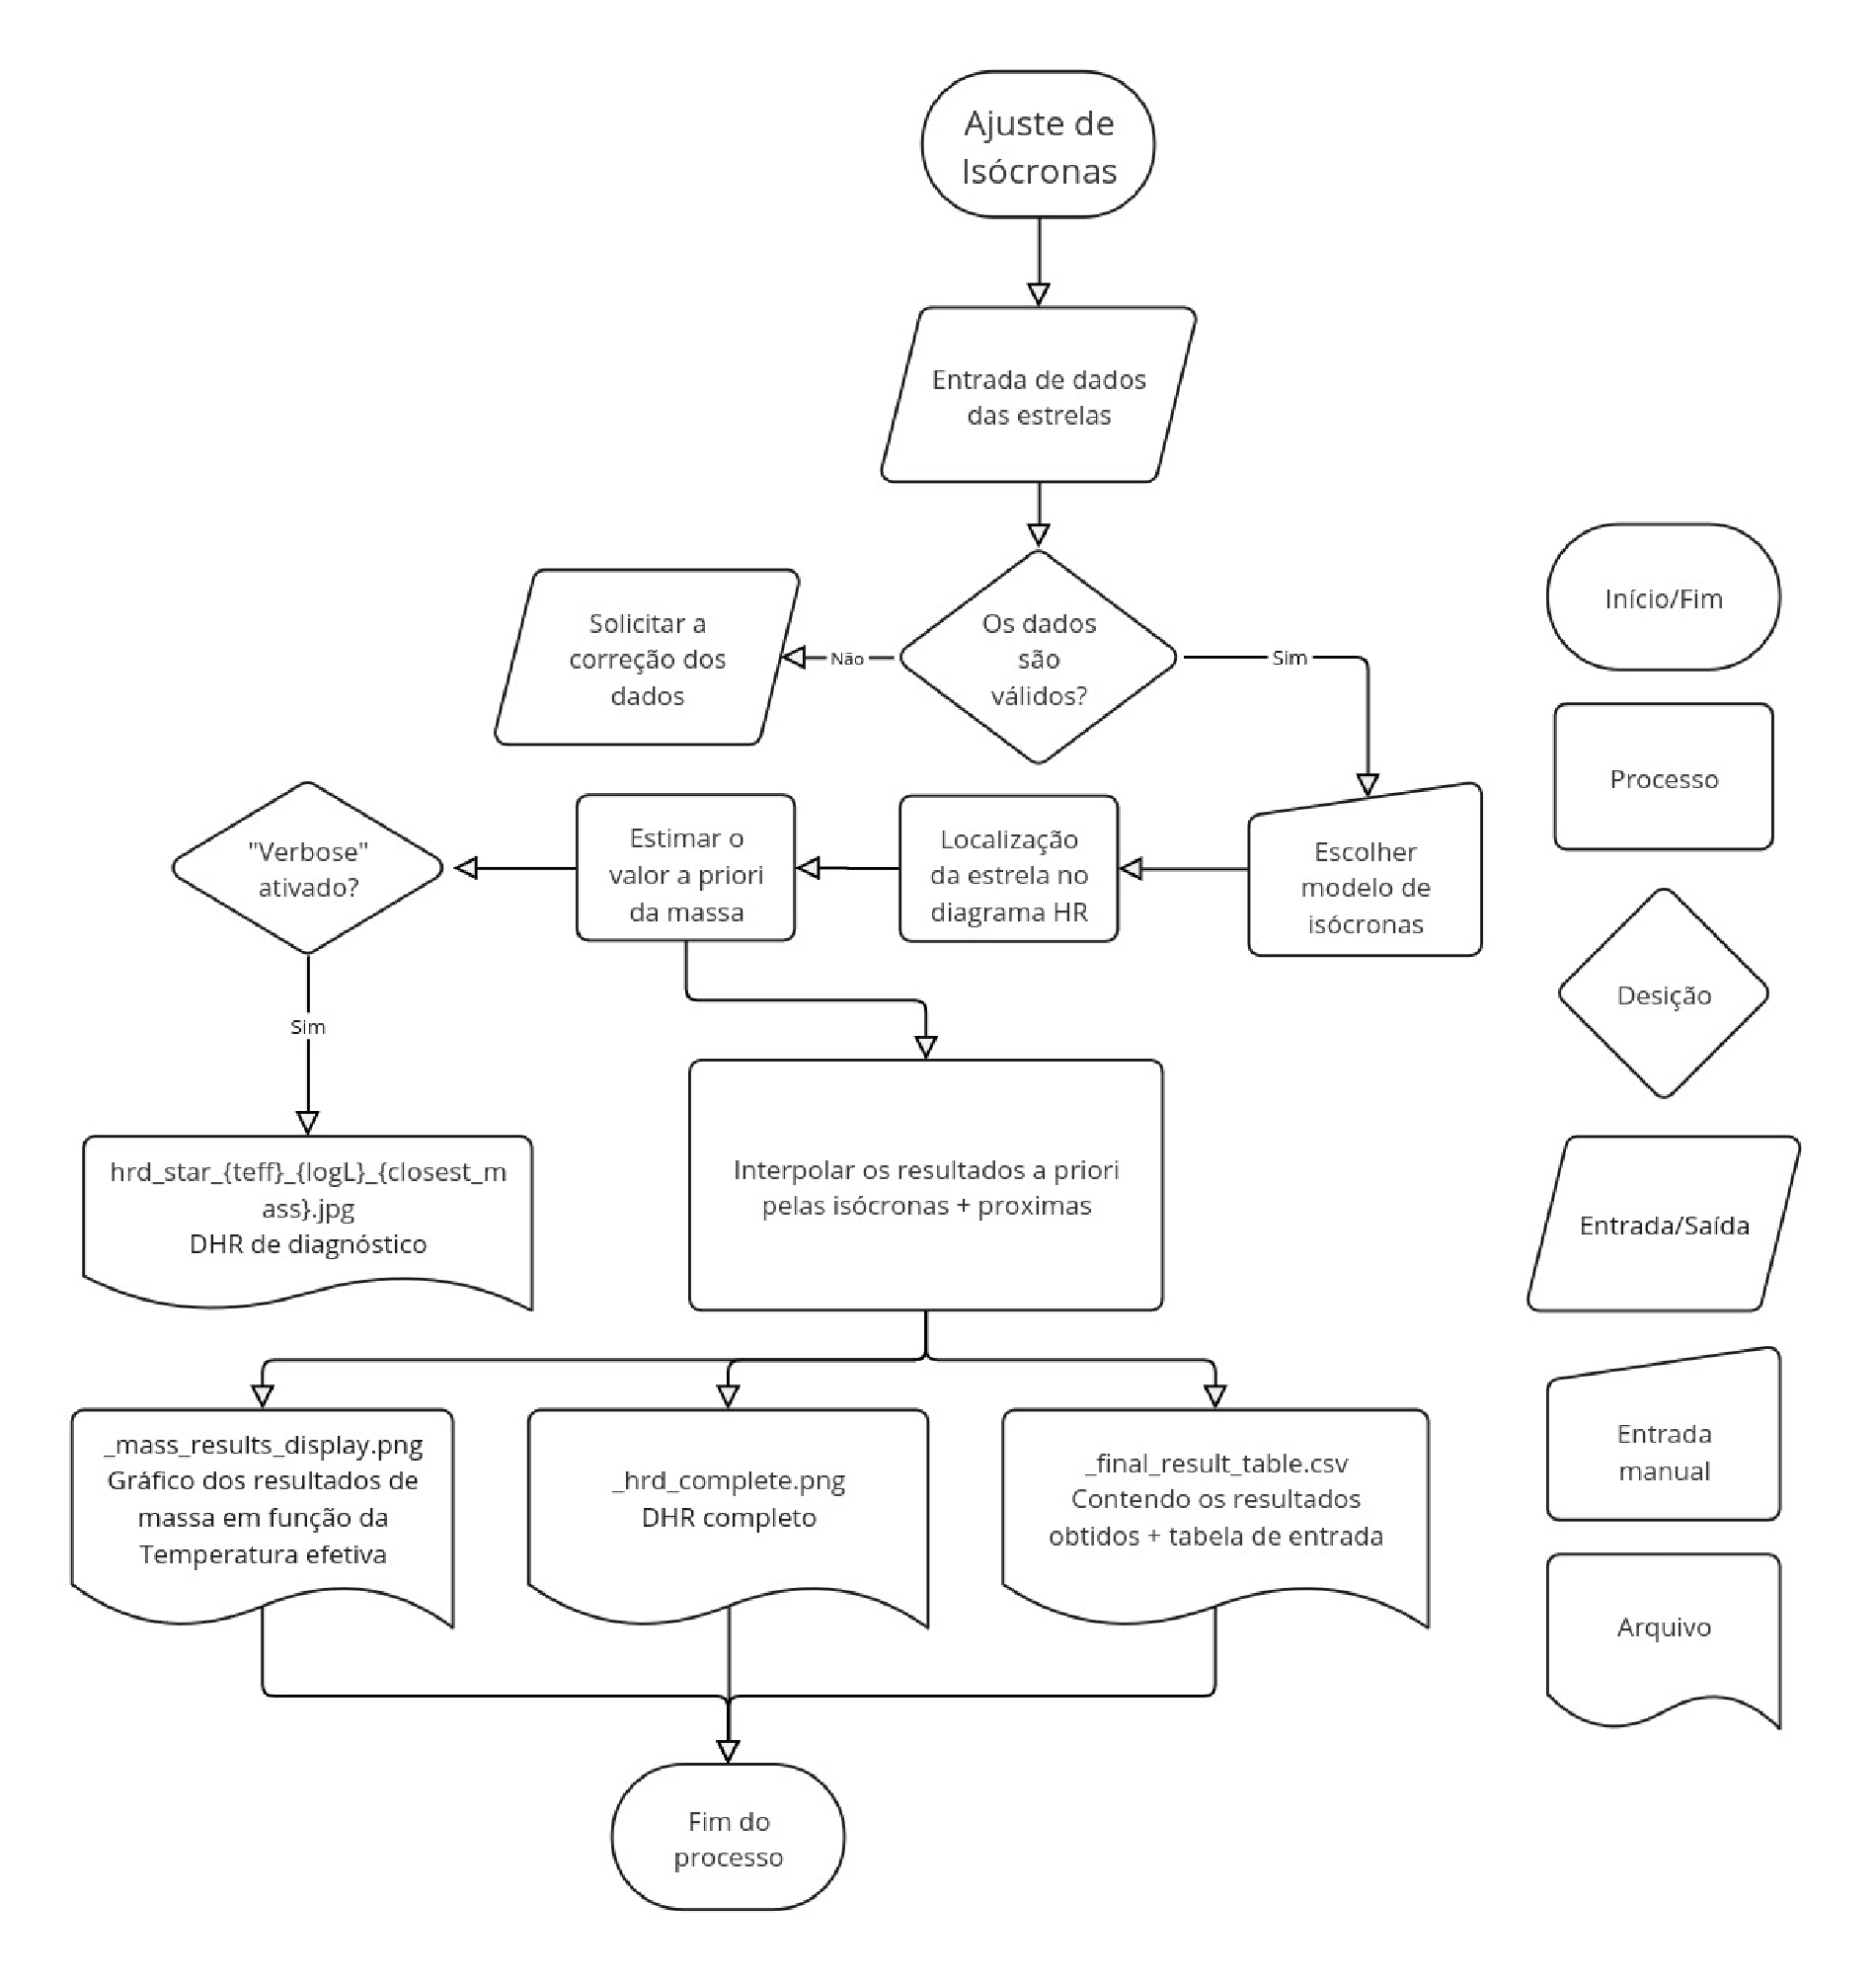
\includegraphics[width=0.7\linewidth]{04-figuras/Flowchart_isocfit.pdf}
        	\label{fig:flowchart_isocfit}
        \end{figure}
        
        Para determinar quais são as isócronas e trilhas mais próximas do objeto, foi desenvolvido um código de minimização baseado na equação,
        
        \begin{equation}
            \label{delta}
            \delta = \sqrt{\left(T_{\text{ef}}-T_{\text{ef},\,0}\right)^2 + (L - L_0)^2}\, .
        \end{equation}
        \noindent onde, \(T_{\text{ef}}\) e \(L\) representam, respectivamente, a temperatura efetiva e a luminosidade obtidas das trilhas evolutivas e das isócronas, e \(T_{\text{ef},\,0}\) e \(L_0\) são os valores de temperatura efetiva e luminosidades calculados a partir das interpolações descritas na Seção \ref{sec:parametros}.
        
        \begin{figure}[!h]
            \centering
            \caption[Determinação de massa utilizando o método de ajuste de isócronas.] {Determinação de massa utilizando o método de ajuste de isócronas. No gráfico está o HRD para uma estrela do ONC.}
            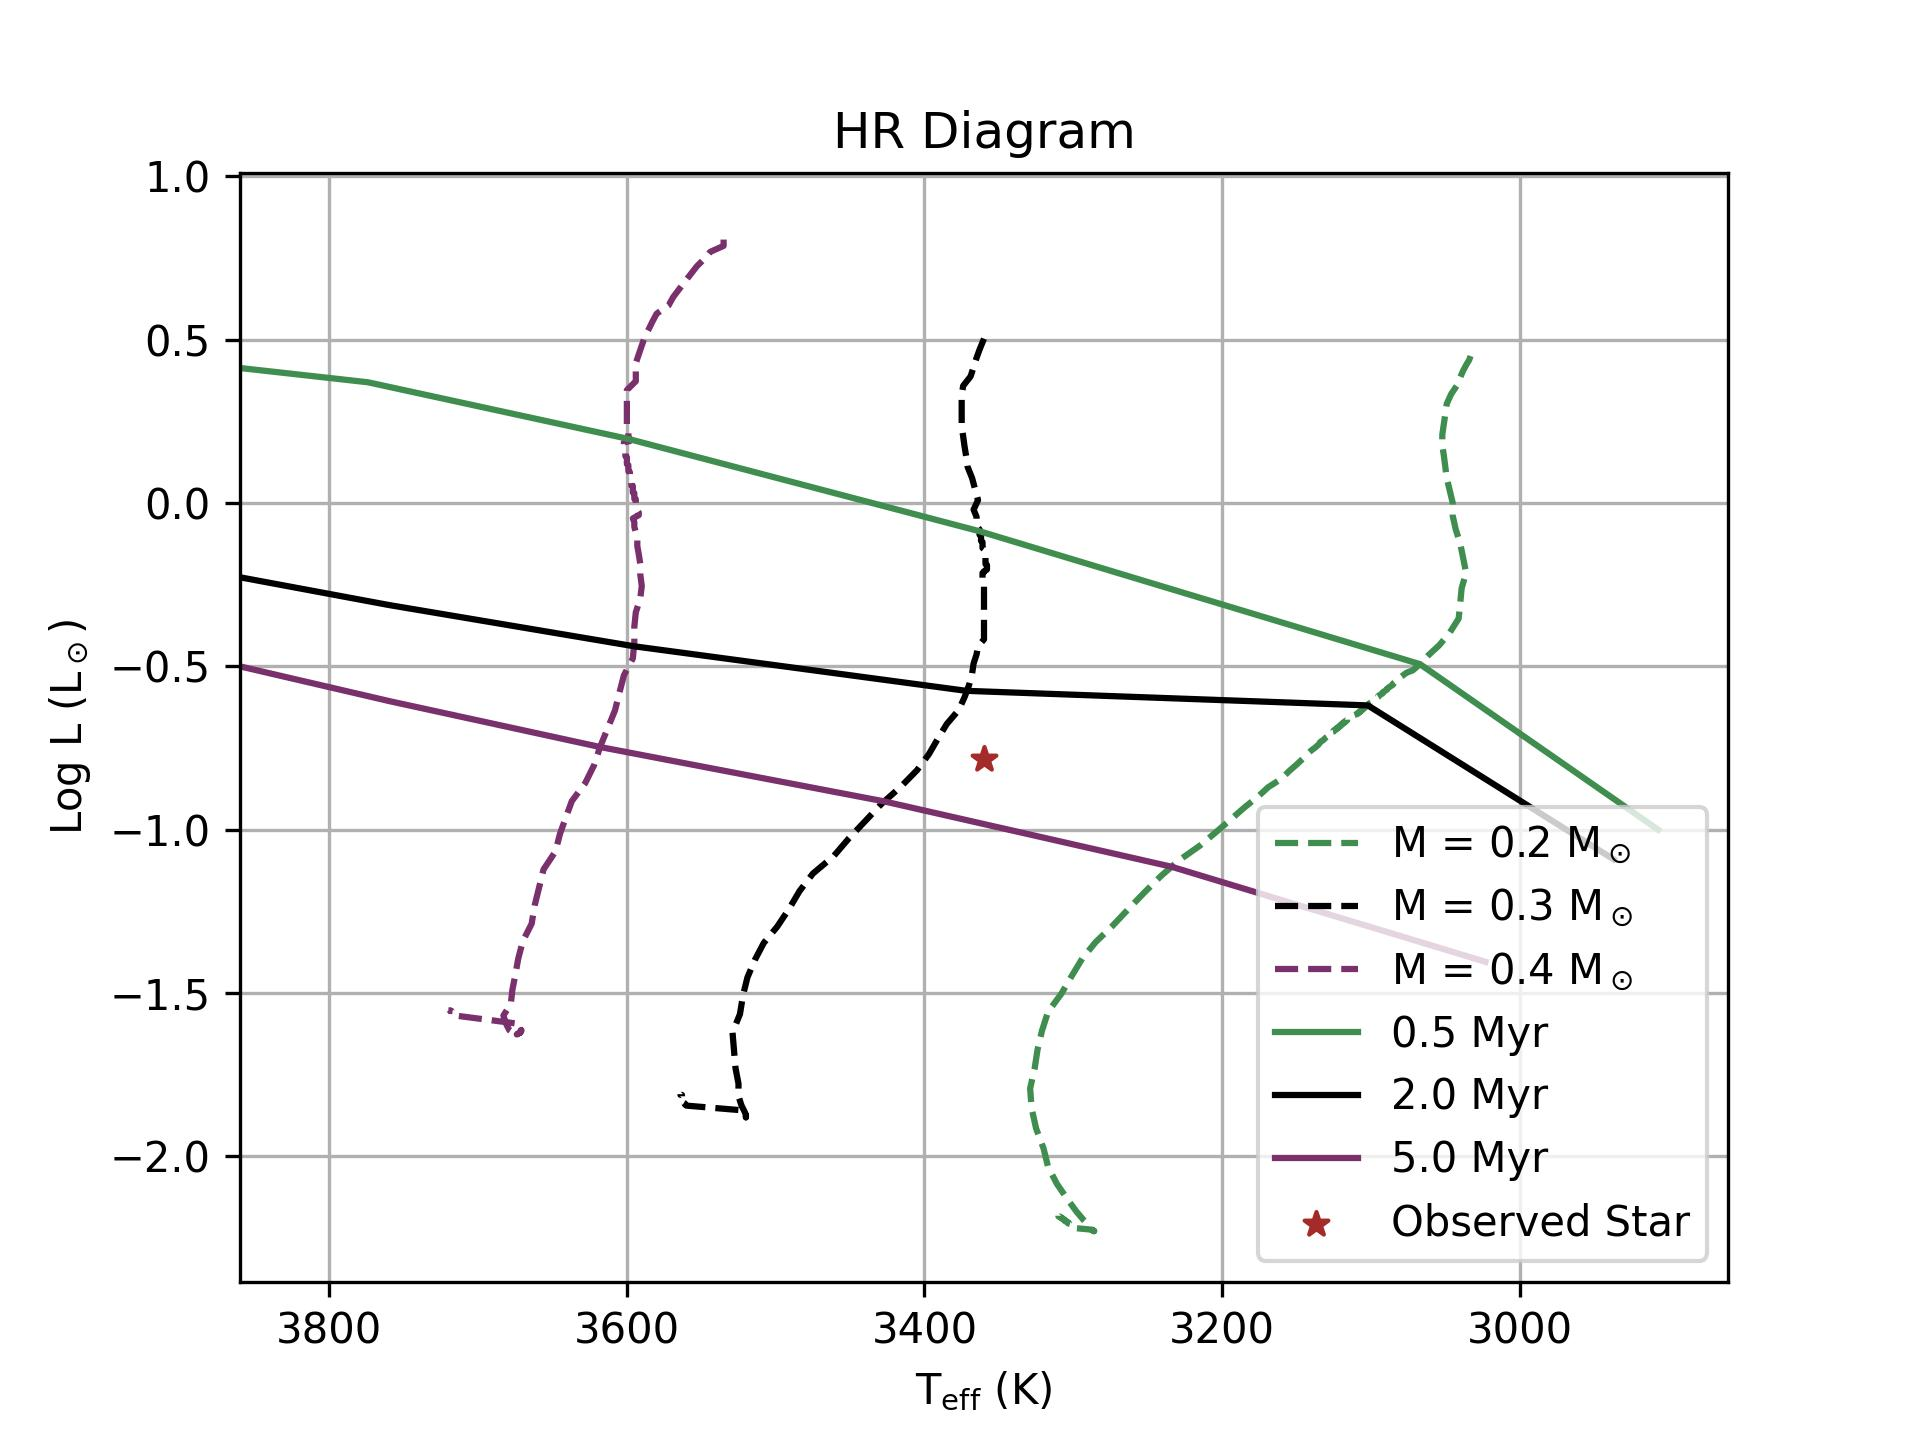
\includegraphics[width=0.5\linewidth]{04-figuras/hrd_star.jpg}
            \label{fig:hrd_isocfit}
        \end{figure}
    
       Seguindo o fluxograma da Figura \ref{fig:flowchart_isocfit}, começamos com a entrada de dados de temperatura efetiva e luminosidade. Após a entrada de dados, o processo continua com a localização da estrela no HRD, como ilustrado na Figura \ref{fig:hrd_isocfit}, onde traçamos as isócronas e trilhas evolutivas do modelo teórico escolhido, mais próximas aos valores de temperatura efetiva e luminosidade da estrela do aglomerado (T0, L0) para a qual se quer calcular a massa. Quando possível, foram traçadas as curvas vizinhas, tanto da trilha evolutiva quanto da isócrona mais próxima, como mostrado no exemplo da Figura \ref{fig:hrd_isocfit}.
       
       O código retorna uma primeira estimativa dos valores de massa e idade de cada objeto. Contudo, a massa e idade verdadeiras provavelmente serão um pouco distintas dos valores obtidos nessa estimativa inicial. Em seguida, a partir dos dados das trilhas evolutivas e isócronas mais próximas da primeira estimativa, e os dados das isócronas e trilhas vizinhas, foi realizada uma interpolação da massa pela temperatura efetiva dessas isócronas para refinar e obter assim o valor final. 
       
       Por fim, um HRD completo, uma exibição de resultados de massa em função da temperatura efetiva e uma tabela com os resultados são salvos separadamente, permitindo a análise e a visualização eficientes dos parâmetros estelares envolvidos no processo.

        A localização precisa no HRD depende de estimativas precisas de extinção e temperatura efetiva (\(T_{ef}\)). Se a extinção ou \(T_{ef}\) estiverem erradas, isso obviamente introduzirá erros sistemáticos na localização e, consequentemente nas idades e massas inferidas a partir da comparação com as trilhas evolutivas e isócronas. Para estrelas PMS, erros sistemáticos nas idades podem deslocar sistematicamente as escalas de tempo inferidas para a dissipação do disco protoplanetário e a formação de planetas gigantes, \cite{Herczeg2015}.
        
    \subsection{Relação massa-luminosidade (RML)}\label{subsec:rml}
        As estimativas mais comuns de massa na literatura são baseadas em relações empíricas, como a relação massa-luminosidade. Historicamente, têm sido usado binárias eclipsantes isoladas para construir estes conjuntos de dados de referência,  \cite{serenelli2021weighing}.
        
        Como uma alternativa aos métodos baseados nos dados de estrelas binárias, adotamos uma abordagem semi-empírica, utilizando os dados de modelos de isócronas teóricas, obtidas dos modelos de evolução estelar, que fornecem valores esperados para os parâmetros necessários para construir os modelos de regressão e estimar o valor de massa estelar em cada aglomerado. 
        Para evitar limitações com a disponibilidade de parâmetros necessários para a determinação da luminosidade, os modelos foram construídos a partir da magnitude absoluta, corrigida pela extinção em aglomerados mais jovens dada a influência não uniforme da região de formação estelar, como feito anteriormente quando utilizamos o método descrito na Seção \ref{subsec:isocfit} de ajuste de isócronas
        
        As isócronas utilizadas para construir os modelos de regressão para relações massa-magnitude foram obtidos do modelo BHAC15 a partir da biblioteca \textit{Madys} de \citeonline{squicciarini2022madys}, que oferece uma ferramenta que permite simular estrelas sintéticas a partir dos modelos de evolução estelar.
         
    \subsubsection{Modelagem com Aprendizagem de Máquina}
        A metodologia empregada na utilização da relação massa-magnitude para a determinação da massa de estrelas jovens em aglomerados estelares envolve o uso de técnicas e modelos de aprendizagem de máquina.
        A partir dos dados coletados do modelo de isócronas teóricas, são construídos os modelos de regressão. O aprendizado de máquina permite maior flexibilidade na abordagem de possíveis não linearidades nessa relação, que podem ser negligenciadas pelos métodos paramétricos tradicionais. Ao utilizar vários algoritmos, o modelo visa fornecer estimativas precisas de massa, dentro das limitações esperadas.
        
        Para a utilização dos métodos de aprendizagem de máquina, é preciso separar os dados em, pelo menos, uma amostra de treinamento e outra para testes. Com esta finalidade, utilizamos o \textit{k-fold}, que é uma técnica de reamostragem onde a amostra original é dividida aleatoriamente em k subamostras (frequentemente chamadas de “dobras”) de tamanho igual. Das k subamostras, uma subamostra é mantida como dados de validação para testar o modelo, e as k-1 subamostras restantes são usadas como dados de treinamento. O processo de validação cruzada é então repetido k vezes, usando cada uma das k subamostras exatamente uma vez como dados de validação. Assim, dividimos a amostra dos dados das isócronas teóricas em 10 subconjuntos, um para os testes e nove voltados para o treinamento individual de cada modelo de regressão, a fim de modelar a relação entre massa e magnitude. Avaliando o ajuste com base na pontuação de precisão da validação cruzada\footnote{ A validação cruzada é uma técnica de validação comumente utilizada para avaliar modelos de treinando construídos a partir de aprendizagem de máquina. Dividindo os dados de teste em subconjuntos e avaliando-os no subconjunto complementar dos dados, a validação cruzada é usada para detectar o superajuste, ou seja, a falha na generalização de um padrão e o sub-ajuste, a falha na capacidade de reproduzir o padrão.} assegura-se que os modelos não estão superajustando\footnote{ Superajuste (overfitting) ocorre quando um modelo de aprendizado de máquina captura o ruído dos dados de treinamento como se fosse um sinal genuíno. Em outras palavras, o modelo se torna muito complexo e se ajusta demais aos dados de treinamento, perdendo sua capacidade de generalizar para dados não vistos.} os dados de treinamento. Com um espaço de hiper parâmetros para cada modelo de regressão otimizados por meio de buscas em grade (grid search) que minimize o valor do resíduo quadrático médio negativo (NMSE), cada modelo foi ajustado utilizando o melhor conjunto de hiper parâmetros.
        
        \begin{figure}[!h]
        	\centering
        	\caption[Fluxograma do processo de ajuste de isócronas.] {Fluxograma do processo de relação massa-magnitude (RMM) para estimativa de massa estelar.}
        	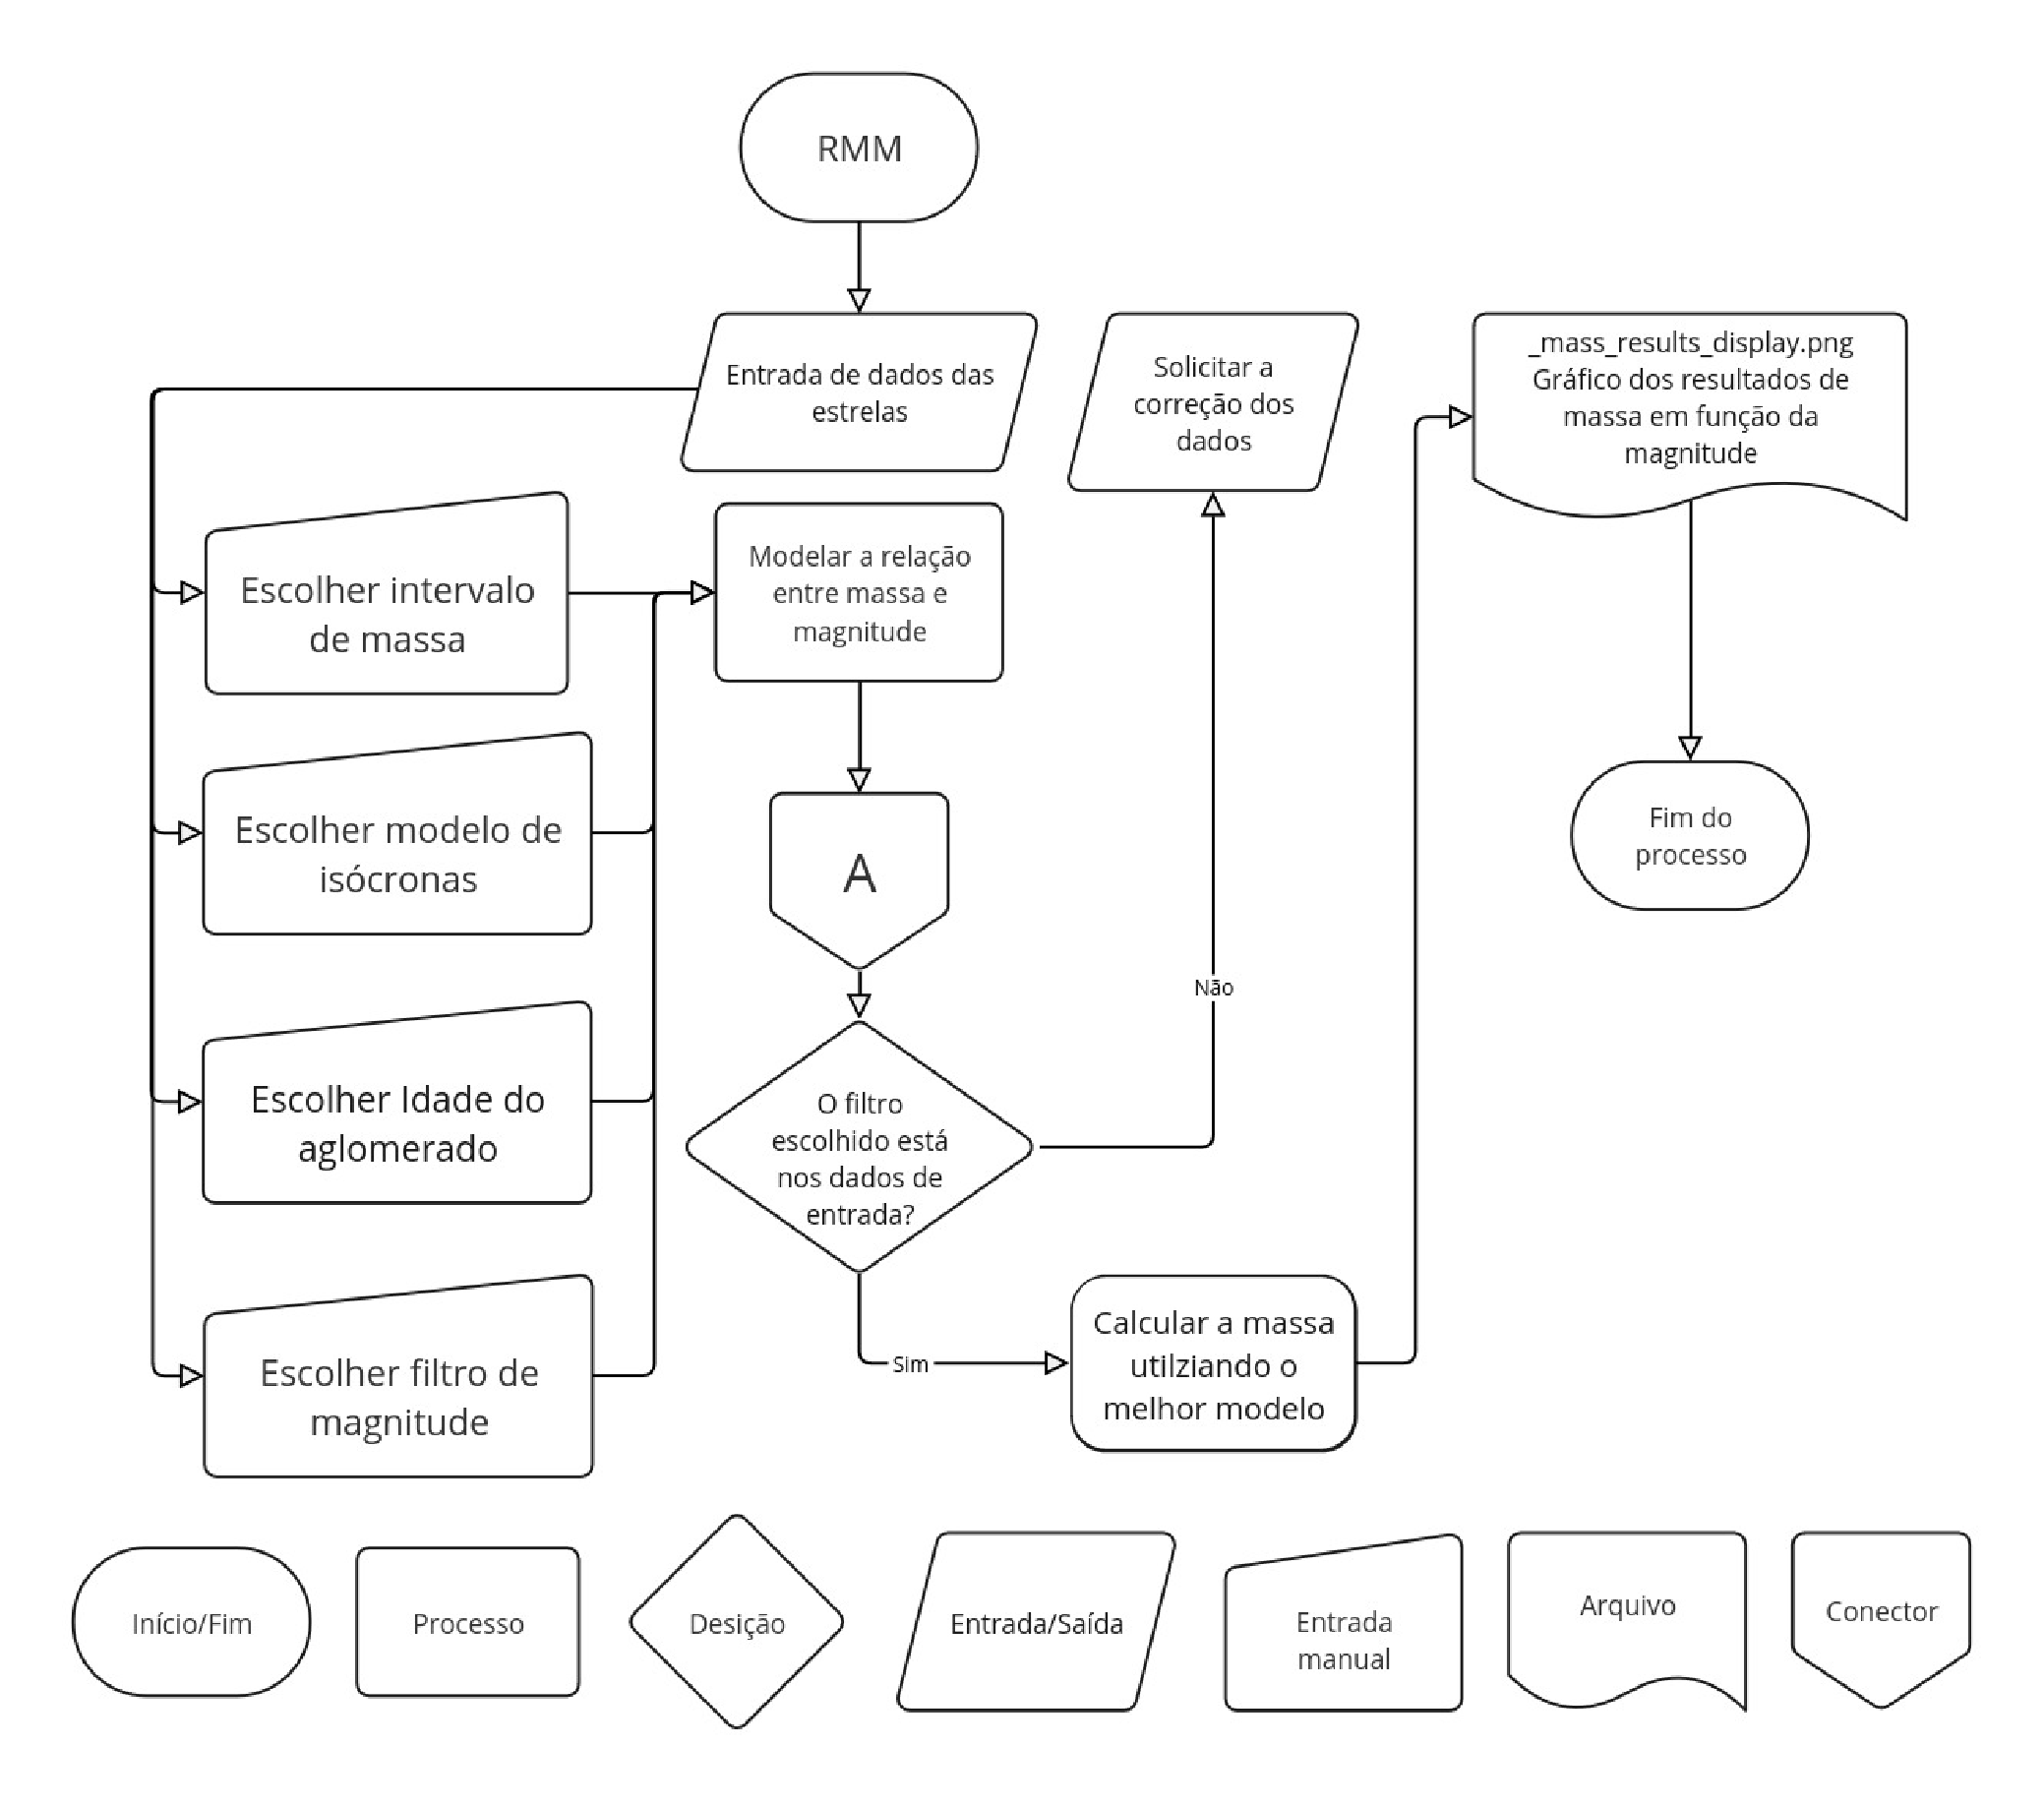
\includegraphics[width=0.7\linewidth]{04-figuras/Flowchart_rmm_a.pdf}
        	\label{fig:flowchart_rmm_a}
        \end{figure}
        
        O fluxograma da Figura \ref{fig:flowchart_rmm_a} ilustra esse processo da estimativa da massa estelar usando a Relação Massa-Magnitude (RMM). O processo começa com a entrada dos dados de magnitude, seguida pela definição de parâmetros específicos, como o intervalo de massa, o modelo de isócronas, a idade do aglomerado e o filtro de magnitude. Uma relação entre massa e magnitude é então modelada usando diferentes métodos de ajuste. O processo prossegue para calcular a massa estelar usando o modelo ideal. O resultado final é um gráfico que mostra os resultados de massa como uma função da magnitude, o que ajuda a visualizar e validar a estimativa de massa.
        
        As técnicas de regressão baseadas em aprendizado de máquina visam ajustar modelos que minimizem a raiz do resíduo quadrático médio (RMSE), dado pela equação (\ref{sr}).

         \begin{equation}
            \label{sr}
            RMSE = \sqrt{\frac{1}{k}\sum_{j=0}^{k} [f(x_j) - y_j]^2} \, ,
        \end{equation}
        \noindent aqui, \( f \) representa a função de regressão que estima \( y_j \) a partir dos dados de entrada \( x_j \). A escolha de \( f \) varia entre os diferentes métodos de regressão disponíveis na biblioteca \textbf{Scikit-Learn}, do \textit{python}, listados abaixo:
        
        \begin{itemize}
            \item[(i)] \textbf{Regressão Linear}: Técnica básica de regressão que modela a relação entre uma variável dependente e uma ou mais variáveis independentes mediante uma equação linear, servindo como modelo de referência para comparação com técnicas mais complexas.
            Em acréscimo, foram construídos modelos de regressão linear baseados nas funções de perda Ridge, Lasso e a técnica de rede elástica (ElasticNet), que combina as duas.
            
            \item[(ii)] \textbf{Regressão Bayesiana}: O algoritmo Naive Bayes é um tipo de técnica de aprendizado supervisionado que é comumente usado para tarefas de classificação e regressão. Esse algoritmo funciona utilizando o teorema de Bayes para prever um novo ponto com base na amostra de dados atribuída.
            
            \item[(iii)] \textbf{Regressão de Vetores de Suporte (Support Vector Regressor, SVR)}: Método de regressão que utiliza uma função de kernel para capturar relações não lineares nos dados. SVR busca encontrar uma função que tenha no máximo uma margem de erro \(\varepsilon\) para cada ponto de treinamento. Selecionado pela sua capacidade de lidar com dados não lineares e seu bom desempenho em problemas de regressão com muitos atributos.

            \item[(iv)] \textbf{Árvore de Decisão (Decision Tree)}: Uma árvore de decisão é um dos mais poderosos algoritmos de aprendizado supervisionado usado para resolver problemas de regressão e classificação.
            Trata-se de uma estrutura semelhante a um fluxograma, em que cada nó interno representa um “teste” em um atributo, cada ramo representa o resultado do teste e cada nó folha representa um valor numérico (na regressão).
            
            \item[(v)] \textbf{Floresta Aleatória (Random Forest)}:
            Ao usar árvores de decisão, existe o risco de superajuste, por ser fácil para a árvore se tornar muito complexa e se ajustar às especificidades dos pontos de dados individuais em vez das características gerais das distribuições das quais eles são extraídos. Uma floresta aleatória é um meta-estimador que ajusta vários modelos de regressão de árvores de decisão em várias subamostras do conjunto de dados e usa o cálculo da média para melhorar a precisão da previsão e controlar o excesso de ajuste.

            \item[(vi)] \textbf{Impulsionamento em Gradiente}: Esse estimador constrói um modelo aditivo em um estágio avançado ele permite a otimização de funções de perda diferenciáveis arbitrárias. A cada passo, uma árvore de regressão é ajustada no gradiente negativo da função de perda fornecida, com os gradientes representando as derivadas parciais da função de perda em relação aos parâmetros do modelo, indicando a direção e a taxa de mudança necessária para reduzir a perda. 
            
            \item[(vii)] \textbf{Impulsionamento Ada}: Um modelo de regressão AdaBoost é um meta-estimador que começa ajustando um modelo no conjunto de dados original e, em seguida, ajusta cópias adicionais do modelo no mesmo conjunto de dados, mas onde os pesos das instâncias são ajustados conforme o erro da previsão atual. Dessa forma, os modelos de regressão subsequentes se concentram mais em casos difíceis.

             \item[(viii)] \textbf{K-ésimos Vizinhos mais Próximos (K-Nearest Neighbors)}: O alvo é previsto pela interpolação local dos alvos associados aos vizinhos mais próximos no conjunto de treinamento.

             \item[(ix)] \textbf{Rede Elástica (ElasticNet)}: A regressão linear de rede elástica combina as penalidades das funções Lasso e Ridge para normalizar os modelos de regressão, diminuindo o possível viés e variância.
        \end{itemize}

        
    \subsubsection{Ferramentas estatísticas e análise dos resultados}\label{sec:estatistica}
        A probabilidade e a estatística ganham espaço quando não há completude de informação acerca das condições iniciais de um sistema.
        
        O processo de avaliação de modelos para estimar a massa estelar passa por esse crivo estatístico, resumido no fluxograma da Figura \ref{fig:flowchart_rmm_b}, começando com a geração de estrelas sintéticas com base no modelo de isócronas selecionado. Os dados são divididos em conjuntos de treinamento e teste, e cada modelo é treinado com ajuste de hiper parâmetro por meio da busca de grade.
        
        \begin{figure}[!h]
        	\centering
        	\caption[Fluxograma do processo de treinamento e avaliação de modelos.] {Fluxograma do processo de treinamento e avaliação de modelos na estimativa de massa estelar.}
        	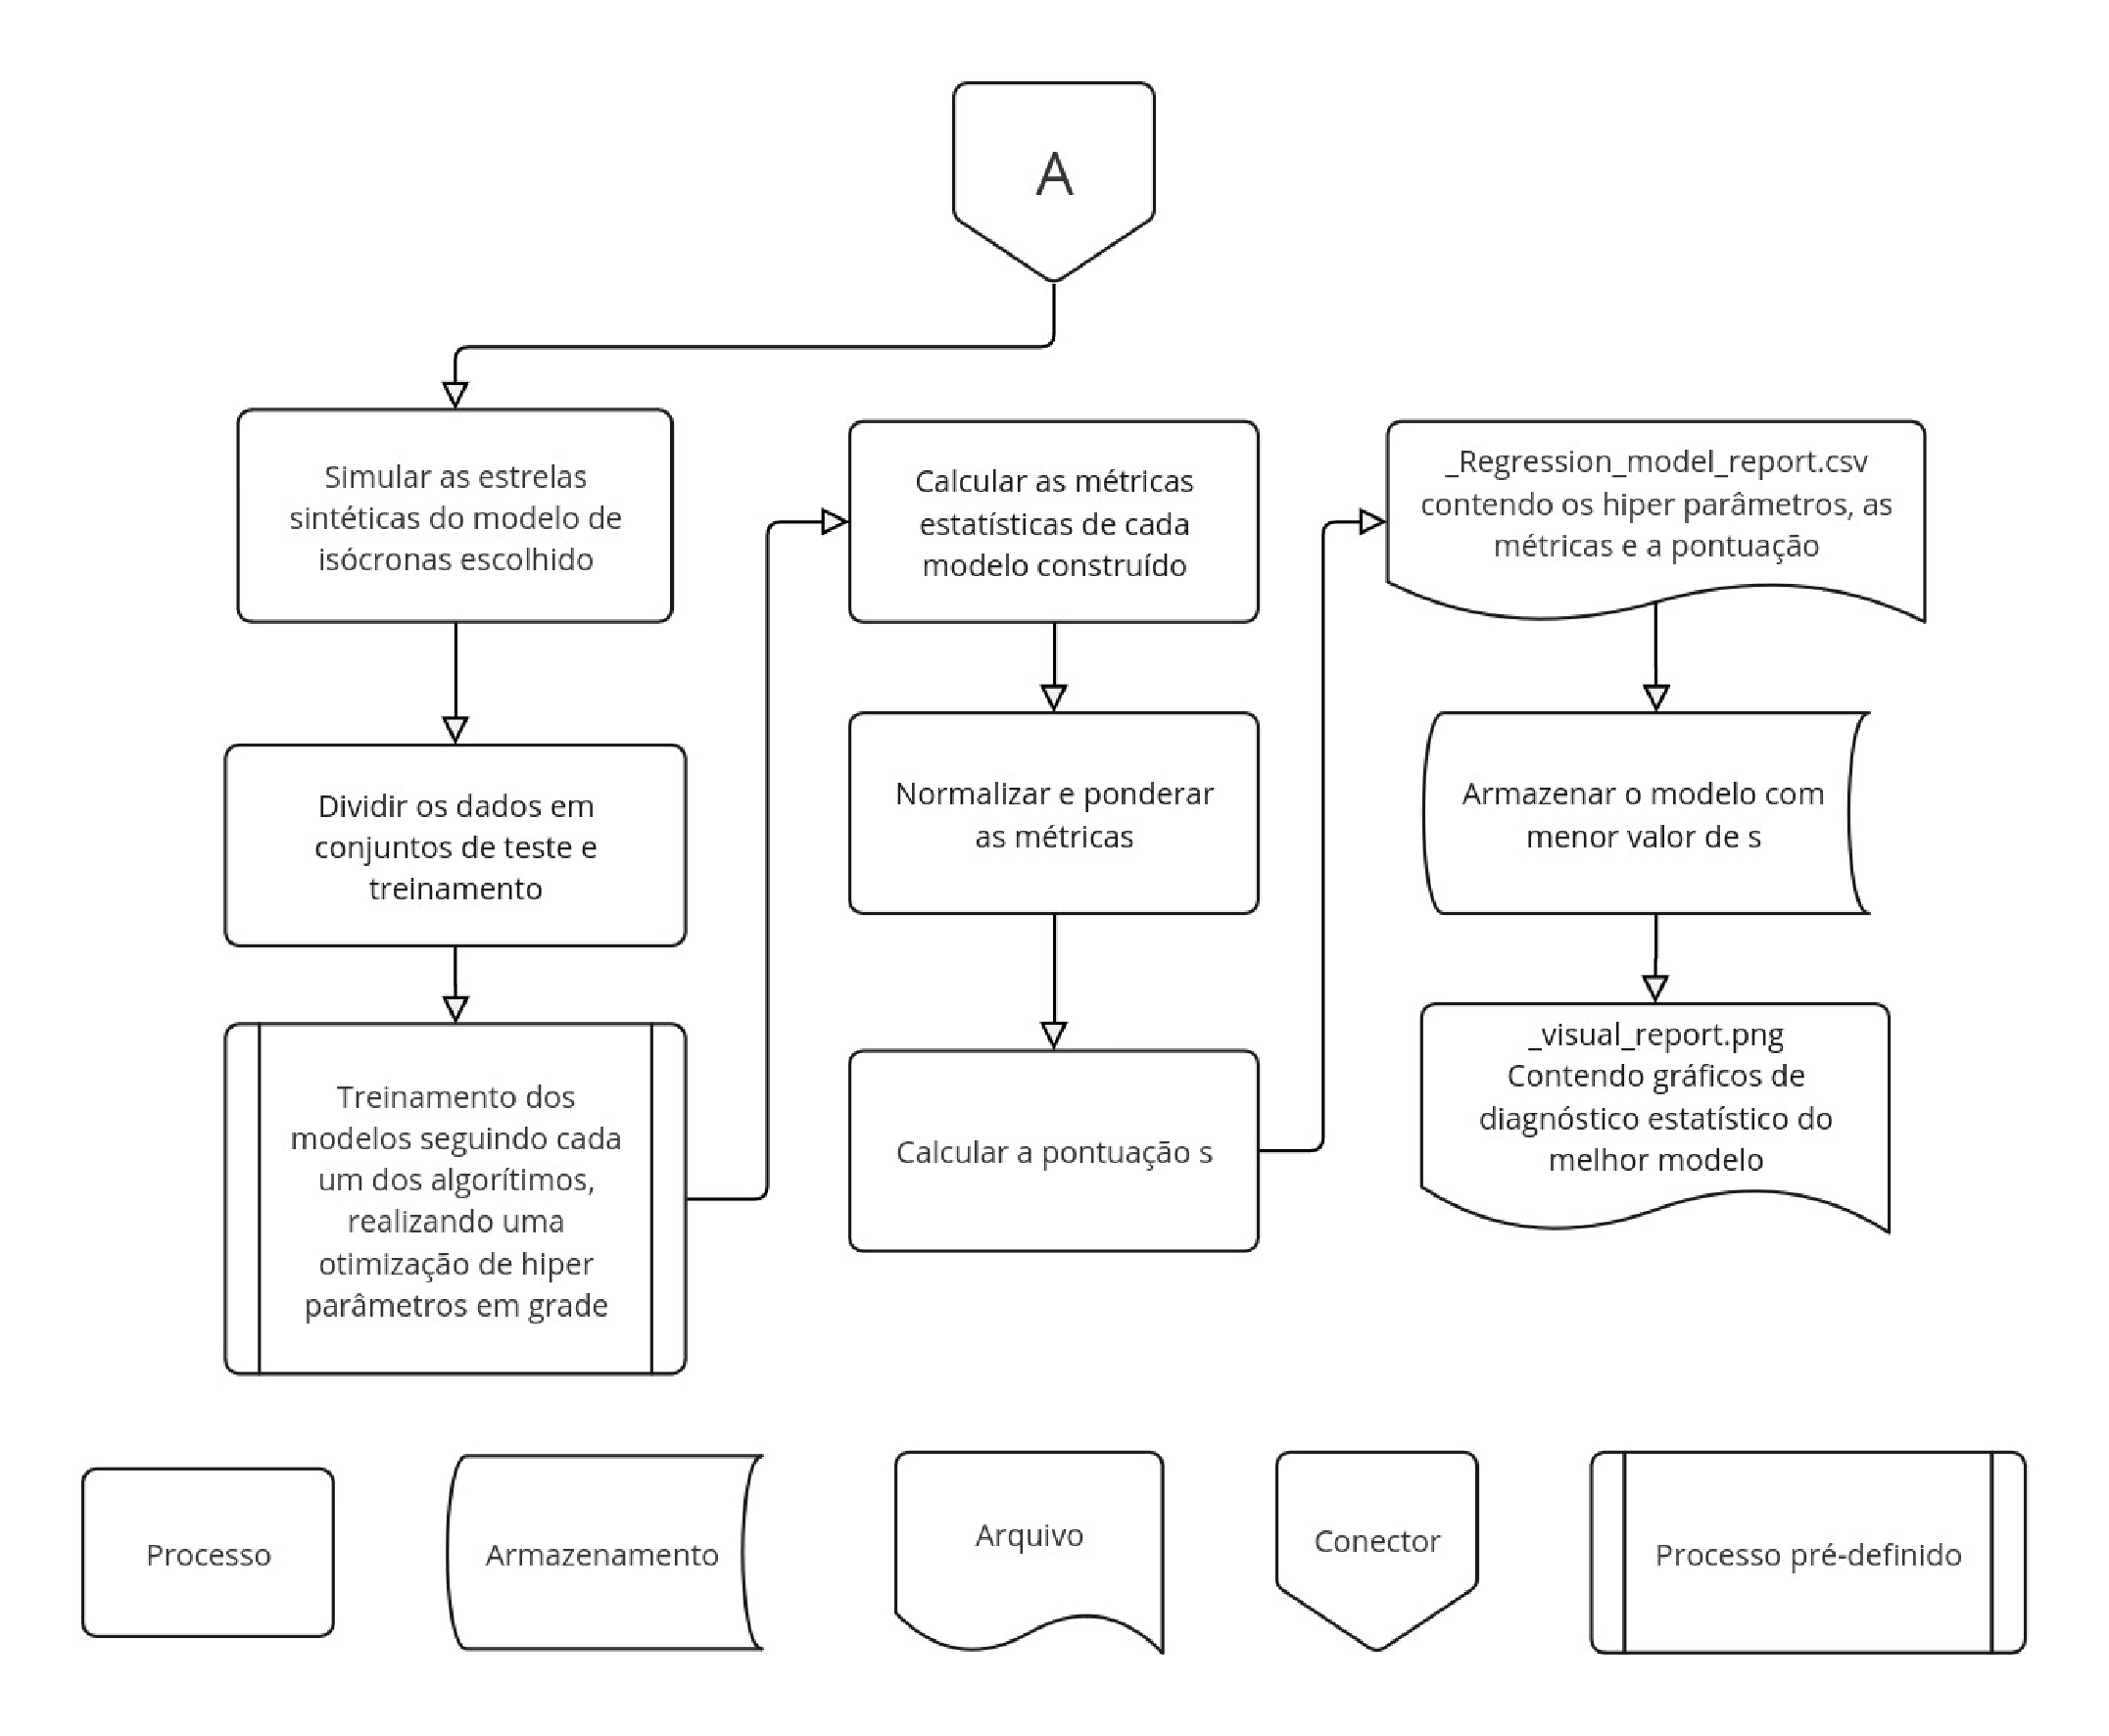
\includegraphics[width=0.7\linewidth]{04-figuras/Flowchart_rmm_b.pdf}
        	\label{fig:flowchart_rmm_b}
        \end{figure}
        
        Para avaliar a qualidade dos modelos treinados, introduzimos métricas essenciais como a RMSE, cuja função de perda está associada à otimização dos modelos de regressão, o erro absoluto médio (Mean Absolute Error, MAE), que exerce a mesma função, o coeficiente de determinação (\(R^2\)) e o Critério de Informação de Akaike (Akaike's Information Criterion, AIC). O AIC é uma métrica baseada na teoria da informação que avalia a qualidade de um modelo estatístico considerando tanto o ajuste aos dados quanto sua simplicidade. Ele é definido matematicamente como:
        
        \begin{equation}\label{AIC}
   		        \text{AIC} = 2k - 2\ln(\mathcal{L}),
   		 \end{equation}

        \noindent onde \(k\) é o número de parâmetros estimados no modelo e \(\mathcal{L}\) é a máxima verossimilhança do modelo ajustado. O AIC penaliza modelos mais complexos (com maior \(k\)) para evitar superajuste, permitindo a comparação entre modelos concorrentes. Modelos com valores de AIC menores são considerados melhores. Para isso, a amostra dos dados teóricos retirados dos modelos de isócronas utilizados é dividida em duas amostras, uma para treinar os modelos e a outra para validar a qualidade dos mesmos a partir das métricas discutidas.
        
        Adicionalmente, foi realizado uma análise comparativa utilizando o método de regressão linear por mínimos quadrados ordinários (OLS), disponível na biblioteca \textbf{Statsmodels} do \textit{python} entre os dados de treino e teste.
        
         Em seguida, o processo calcula um conjunto de métricas estatísticas para cada modelo, definindo, a matriz das métricas \(\mathcal{M}\), onde cada linha representa um dos algoritmos discutidos anteriormente, conforme apresentado na equação (\ref{matrix:metric}), e a matriz de pesos \(\mathcal{P}\) adotada, cujos valores são definidos com base na magnitude dos valores possíveis. Esses pesos refletem a relação entre a qualidade do ajuste — indicada pelos erros RMSE e MAE — e a compatibilidade do modelo construído com o modelo de isócronas teóricas utilizado, representada pelo coeficiente de determinação (\(R^2\)) e pelo (AIC). A relação entre esses dois conjuntos de indicadores é estabelecida em uma proporção de 60-40. A matriz dos pesos utilizados está apresentada na equação (\ref{matrix:pesos}).
        
        
        \begin{equation}
        \label{matrix:metric}
            \mathcal{M}=\begin{bmatrix}
                {RMSE}_{1} & {MAE}_{1} & (1 - {R^2}_{1}) & {AIC}_{1} \\
                {RMSE}_{2} & {MAE}_{2} & (1 - {R^2}_{2}) & {AIC}_{2} \\
                \vdots & \vdots & \vdots & \vdots \\
                {RMSE}_{n} & {MAE}_{n} & (1 - {R^2}_{n}) & {AIC}_{n}
            \end{bmatrix}
        \end{equation}
        
        \begin{equation}
        \label{matrix:pesos}
            \mathcal{P}=\begin{bmatrix}
                0.35 & 0.25 & 0.30 & 0.10  
            \end{bmatrix}
        \end{equation}
    	 Para automatizar a escolha do melhor modelo construído a partir das relações entre massa e magnitude utilizando diferentes métricas, definimos uma nova métrica: a pontuação \(\mathcal{S}\), dada pela equação (\ref{eq:score}), onde as métricas são normalizadas e ponderadas, especialmente porque o valor do coeficiente de determinação (\(R^2\)) varia de modo inverso aos demais e o critério de informação de Akaike pode assumir valores negativos.
        
        \begin{equation}
            \label{eq:score}
            \mathcal{S} = \mathcal{\hat{M}} \cdot \mathcal{P}^T
        \end{equation}
       \noindent onde \(\mathcal{\hat{M}}\) é a matriz normalizada das métricas. Para se construir os elementos normalizados da matriz \(\mathcal{M}\) utilizamos a equação abaixo: 
        
        \begin{equation}
            \label{eq:norm}
            \hat{x} = \frac{x - x_{min}} {x_{max} - x_{min}} \, ,
        \end{equation}
    	\noindent onde \textit{x} é o elemento da matriz \(\mathcal{M}\) de cada métrica, \(\,x_{min}\,\) o menor e \(\,x_{max}\,\) o maior valor obtido nessa matriz, retornando o valor normalizado \(\hat{x}\).
        
        A menor pontuação (\textit{s}) da matriz \(\mathcal{{S}}\) indica o melhor modelo. Esse modelo é então armazenado, e um relatório dos modelos de regressão treinados, contendo hiper parâmetros, métricas e pontuações é salvo em um arquivo. Além disso, uma imagem contendo um relatório visual com gráficos de diagnóstico para o melhor modelo é salvo como um arquivo PNG. Nos casos de possíveis degenerescências nos resultados, foi adotado o modelo mais simples. Assim, é realizado o treinamento do melhor modelo otimizado utilizando a amostra total dos dados do modelo de evolução adotado.

        Essa abordagem permite uma comparação direta entre modelos, considerando um conjunto de métricas relevantes. Para verificar a adequação do melhor modelo gerado para o aglomerado estudado, utilizaremos os seguintes conceitos:
        
        \begin{itemize}
            \item[(i)] \textbf{Correlação}: 
            o coeficiente de determinação (\(R^2\)) mede o quanto a variabilidade da variável dependente do modelo em relação aos dados originais é explicada pelas variáveis independentes. Essa estatística é amplamente utilizada em modelos estatísticos cujo objetivo principal é prever resultados futuros ou testar hipóteses com base em informações relevantes. Em essência, o \(R^2\) indica o quão bem o modelo reproduz os resultados observados, ao representar a proporção da variação total nos resultados que o modelo consegue explicar. Além disso, fornece uma medida do grau de correlação entre os dados e o modelo ajustado.
            
            \item[(ii)] \textbf{Normalidade dos Resíduos}:
            a normalidade dos resíduos, indicada pelos testes, assegura que o modelo está captando bem os padrões dos dados, de forma que todo e qualquer erro associado às medidas é de natureza aleatória e não do modelo.
            
            \item[(iii)] \textbf{Cedasticidade}: a razão entre as variâncias de duas amostras categoriza a cedasticidade em dois tipos: homoscedasticidade e heteroscedasticidade. Quando a variância é homogênea, tendo a razão \(\approx 1\), a distribuição é considerada homoscedástica, pois se mantém semelhante na maioria dos pontos. Por outro lado, se a variância varia entre os pontos, a razão entre as variâncias é \(\ll 1\) e a distribuição é classificada como heteroscedástica, indicando que os erros do modelo não apresentam a mesma variância em todos os casos. Comparar os valores calculados com os resíduos absolutos pode revelar uma tendência que ajuda a identificar a natureza dos erros. \\
            Ex: uma reta crescente indica um termo linear positivo.

            \item[(iv)] \textbf{\textit{Outliers} e influência}:
            a identificação de \textit{outliers} é realizada através do resíduo padronizado (\({\sigma}\)) e da distância de Cook (\(D\)) que identifica o grau de influência desses \textit{outliers} no ajuste do modelo. O valor crítico da distância de Cook é comumente adotado como \(D_{crit} = 4\).  Aqui distância de Cook crítica é normalizada a partir da razão do tamanho da amostra: \(\hat{D}_{crit} = D_{crit} / (n-2)\)
    
        \end{itemize}
        
        Para a análise comparativa, o valor de \(R^2\) é crucial para avaliar a proximidade do ajuste do modelo com os dados referenciais, sendo um valor próximo de 1 indicativo de uma forte correlação. Neste estudo, dados com \(R^2 \geq 0.75\) foram aceitos como fortemente correlacionados.
        
        Realizamos o teste de normalidade nos resíduos, para aferir se os erros associados à comparação são de natureza aleatória, ou se são causadas por algum viés. Utilizamos o teste de Jarque-Bera, indicado para amostras grandes (\(n \geq 500\)), cuja hipótese nula é a normalidade dos dados. Um p-valor\footnote{O p-valor é a probabilidade de se obter resultados de teste tão extremos quanto o resultado realmente observado, sob a suposição de que a hipótese nula esteja correta.} inferior ao nível de significância\footnote{ O nível de significância é um corte adotado para julgar um resultado como estatisticamente significativo.} (\(\alpha = 0.05\)) leva à rejeição da normalidade.
       
	\section{Validação metodológica}\label{sec:validacao}
		
		Para validar os métodos de determinação de massa empregados, foi utilizado um conjunto controle de dados para verificar o desempenho de cada método, comparando os resultados obtidos com os valores deste conjunto. Para associar uma incerteza nas previsões obtidas, a fim de lidar com possíveis empecilhos causados por utilizar os modelos teóricos de isócronas, combinamos a incerteza associada à metodologia empregada e a incerteza esperada para o método empregado, obtida de \citeonline{serenelli2021weighing}, conforme a equação abaixo:
		
		\begin{equation}
			\label{erro}
			u = u_{m} \sqrt{\hat{y}^2 + \sigma^2} \, ,
		\end{equation}
		\noindent onde, \( \hat{y}\) denota a mediana dos resíduos obtidos dos valores de massa determinados para o conjunto de controle, \( \sigma\) representa a variância de cada conjunto de massas estimadas e \( u_m \) denota a incerteza teórica esperada do método. Para relação massa-luminosidade, \(u_m = 0.15\), e para o ajuste de isócronas, \(u_m = 0.10\).
		